% 
%            ,,                                        
%          `7MM            _.o9                                
%            MM                                             
%  ,6"Yb.    MM  ,p6"bo   ,6"Yb.  M"""MMV  ,6"Yb.  `7Mb,od8 
% 8)   MM    MM 6M'  OO  8)   MM  '  AMV  8)   MM    MM' "' 
%  ,pm9MM    MM 8M        ,pm9MM    AMV    ,pm9MM    MM     
% 8M   MM    MM YM.    , 8M   MM   AMV  , 8M   MM    MM     
% `Moo9^Yo..JMML.YMbmd'  `Moo9^Yo.AMMmmmM `Moo9^Yo..JMML.   
% 
% 
% Free and Open-Source template for academic works
% https://github.com/dpmj/alcazar



% ------------------------------------------------------------------------------
% FILES

% Title page
%% 
%            ,,                                        
%          `7MM            _.o9                                
%            MM                                             
%  ,6"Yb.    MM  ,p6"bo   ,6"Yb.  M"""MMV  ,6"Yb.  `7Mb,od8 
% 8)   MM    MM 6M'  OO  8)   MM  '  AMV  8)   MM    MM' "' 
%  ,pm9MM    MM 8M        ,pm9MM    AMV    ,pm9MM    MM     
% 8M   MM    MM YM.    , 8M   MM   AMV  , 8M   MM    MM     
% `Moo9^Yo..JMML.YMbmd'  `Moo9^Yo.AMMmmmM `Moo9^Yo..JMML.   
% 
% 
% Free and Open-Source template for academic works
% https://github.com/dpmj/alcazar


% ------------------------------------------------------------------------------
% Title page

\thispagestyle{empty}

\pagenumbering{roman}
\setcounter{page}{1}


\newgeometry{
    left    = 3.0cm,
    right   = 3.0cm,
    top     = 3.5cm,
    bottom  = 3.5cm
}


\begin{center}
    
\includegraphics[height=15mm]{opening/resources/logos/logo_upv.pdf}
    \hfill
    
\includegraphics[height=15mm]{opening/resources/logos/logo_upv_telcom.pdf}
\end{center}

\vspace*{30mm}

\begin{center}
    \textbf{\large \textsc{{\thesisDegree} in}}\\
    \textbf{\large \textsc{\thesisArea}}
\end{center}

\vspace*{0mm}

\begin{center}
    \textbf{\large \thesisType}
\end{center}

\vspace*{10mm}

\begin{center}
    \setstretch{1.7}
    \textbf{{\LARGE {}``\thesisTitle''}}\\
\end{center}

\vspace*{15mm}

\begin{center}
    {\large \textsc{Academic course:} \thesisAcademicCourse}
\end{center}

\vspace*{15mm}

\begin{center}
    AUTHOR:
    \par
    \textbf{{\large \thesisAuthor}}
\end{center}

\begin{center}
    TUTOR:
    \par
    \textbf{{\large \thesisTutor}}
\end{center}

\begin{center}
    \vspace*{1mm}
    {\large \thesisDepartment}
\end{center}

\newpage
\thispagestyle{empty}
\restoregeometry


% License
%% 
%            ,,                                        
%          `7MM            _.o9                                
%            MM                                             
%  ,6"Yb.    MM  ,p6"bo   ,6"Yb.  M"""MMV  ,6"Yb.  `7Mb,od8 
% 8)   MM    MM 6M'  OO  8)   MM  '  AMV  8)   MM    MM' "' 
%  ,pm9MM    MM 8M        ,pm9MM    AMV    ,pm9MM    MM     
% 8M   MM    MM YM.    , 8M   MM   AMV  , 8M   MM    MM     
% `Moo9^Yo..JMML.YMbmd'  `Moo9^Yo.AMMmmmM `Moo9^Yo..JMML.   
% 
% 
% Free and Open-Source template for academic works
% https://github.com/dpmj/alcazar


%%%%%%%%%%%%%%%%%%%%%%%%%%%%%%%%%%%%%%%%%%%%%%%%%%%%%%%%%%%%%%%%%%%%%%%%%%%%%%%%%%%%%%%%%%%%
% LICENSE

\newpage
\thispagestyle{empty}

\vspace*{\fill}

\begingroup

    \setlength\tabcolsep{0pt}
    \renewcommand*{\arraystretch}{1.4}
    \renewcommand{\baselinestretch}{0.9}\footnotesize  % Comprime space
    
    \noindent
    \begin{tabular}{m{3.5cm} m{11.5cm}}
        
\includegraphics[width=3cm]{opening/resources/license/by-sa.pdf} & {\normalsize {\thesisAuthor} and {\thesisTutor}} \\
    \end{tabular}
    
    \noindent This work is licensed under the Creative Commons Attribution-ShareAlike 4.0 International (CC BY-SA 4.0) license. This is a human-readable summary of (and not a substitute for) the license. You are free to:
    
    \noindent
    \begin{tabular}{m{1.5cm} m{13.5cm}}
        \textbf{Share} & Copy and redistribute the material in any medium or format.\\
        \textbf{Adapt} & Remix, transform, and build upon the material.\\
    \end{tabular}
    
    \vspace{1mm}
    
    \noindent The licensor cannot revoke these freedoms as long as you follow the license terms:
    
    \noindent
    \begin{tabular}{m{1.5cm} m{13.5cm}}
        
\includegraphics[width=2em]{opening/resources/license/by.pdf} & \textbf{Attribution:} You must give appropriate credit, provide a link to the license, and indicate if changes were made. You may do so in any reasonable manner, but not in any way that suggests the licensor endorses you or your use.\\
        
\includegraphics[width=2em]{opening/resources/license/sa.pdf} & \textbf{ShareAlike:} If you remix, transform, or build upon the material, you must distribute your contributions under the same license as the original.
    \end{tabular}
    
    \noindent To view a complete copy of this license, visit 
    \href{https://creativecommons.org/licenses/by-nc-sa/4.0/}{https://creativecommons.org/licenses/by-sa/4.0}

\endgroup


% Give a little credit to the template :)
% It's completely optional, of course ;)

\begingroup

    \vspace*{2mm}

    \setlength\tabcolsep{0pt}
    \renewcommand*{\arraystretch}{1.4}
    \renewcommand{\baselinestretch}{0.9}\footnotesize  % Comprime space
    
    \noindent
    \begin{tabular}{m{3.5cm} m{11.5cm}}
        
\includegraphics[width=3cm]{opening/resources/logos/alcazar.pdf} & \noindent This document has been generated using {\href{https://github.com/dpmj/alcazar}{Alcázar}}, a free and open source {\LaTeX} template for academic works by \href{https://www.linkedin.com/in/dpmj/}{Juan Del Pino Mena}. \\
    \end{tabular}

    

\endgroup




% About the document
% Collaborators, repositories, social networks, links, etc.
% Feel free to edit this doc:
%% 
%            ,,                                        
%          `7MM            _.o9                                
%            MM                                             
%  ,6"Yb.    MM  ,p6"bo   ,6"Yb.  M"""MMV  ,6"Yb.  `7Mb,od8 
% 8)   MM    MM 6M'  OO  8)   MM  '  AMV  8)   MM    MM' "' 
%  ,pm9MM    MM 8M        ,pm9MM    AMV    ,pm9MM    MM     
% 8M   MM    MM YM.    , 8M   MM   AMV  , 8M   MM    MM     
% `Moo9^Yo..JMML.YMbmd'  `Moo9^Yo.AMMmmmM `Moo9^Yo..JMML.   
% 
% 
% Free and Open-Source template for academic works
% https://github.com/dpmj/alcazar

\newpage


\clearpage
\cleardoublepage
\phantomsection

\pagestyle{empty}

\phantomsection
\addcontentsline{toc}{chapter}{About this work}


%%%%%%%%%%%%%%%%%%%%%%%%%%%%%%%%%%%%%%%%%%%%%%%%%%%%%%%%%%%%%%%%%%%%%%%%%%%%%%%%%%%%%%%%%%%%
% ABOUT THE AUTHORS

\begingroup

    \small
    \setlength\tabcolsep{0pt}
    \renewcommand*{\arraystretch}{1}
    
    \noindent
    \begin{tabular}{p{3.5cm} p{11.5cm}}
        \vspace{0mm} 
\includegraphics[width=3cm]{opening/resources/about/kleiner.png} & \vspace{-0.5mm} {\large \thesisAuthor} 
        \newline A short paragraph about you and how handsome and hard-working you are. Brag about your work, awards, publications and merits. The glory is yours! Congratulations. The Lorem ipsum dolor sit amet, consectetur adipiscing elit. Integer tempus quis elit id sagittis. Cras tincidunt nisi at tellus luctus, et congue dolor posuere. Aliquam suscipit felis sit amet lacus ultrices aliquet. Sed sagittis ultrices nisi, vel elementum elit dignissim non. 
        \vspace{2mm} 
        \newline
        \href{https://orcid.org/}{  % Link to your orcid
            \icon{\faOrcid}{10}{orcid-green}
        }
        \href{https://www.linkedin.com/}{  % Link to your linkedin
            \icon{\faLinkedinIn}{10}{linkedin-blue}
        }
        \href{https://github.com/}{  % Link to your github
            \icon{\faGithub}{10}{github-black}
        }
        \href{https://twitter.com/}{  % Link to your twitter
            \icon{\faTwitter}{10}{twitter-blue}
        }
        \href{mailto:example@domain.org}{  % Your E-mail
            \icon{\faEnvelope}{10}{email-red}
        }
        \href{https://t.me/}{  % Link to your telegram
            \icon{\faTelegramPlane}{10}{telegram-blue}
        }
    \end{tabular}
    
    \vspace{10mm}
    
    \noindent
    \begin{tabular}{p{3.5cm} p{11.5cm}}
        \vspace{0mm} 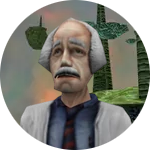
\includegraphics[width=3cm]{opening/resources/about/coomer.png} & \vspace{-0.5mm} {\large \thesisTutor} 
        \newline What a big fish you've got yourself. Show off your tutor. Now that's a job well done. Lorem ipsum dolor sit amet, consectetur adipiscing elit. Integer tempus quis elit id sagittis. Cras tincidunt nisi at tellus luctus, et congue dolor posuere. Aliquam suscipit felis sit amet lacus ultrices aliquet. Sed sagittis ultrices nisi, vel elementum elit dignissim non. Fusce faucibus ex at massa ultrices elementum.
        \vspace{2mm} 
        \newline
        \href{https://orcid.org/}{  % Link to your orcid
            \icon{\faOrcid}{10}{orcid-green}
        }
        \href{https://www.linkedin.com/}{  % Link to your linkedin
            \icon{\faLinkedinIn}{10}{linkedin-blue}
        }
        \href{https://github.com/}{  % Link to your github
            \icon{\faGithub}{10}{github-black}
        }
        \href{https://twitter.com/}{  % Link to your twitter
            \icon{\faTwitter}{10}{twitter-blue}
        }
        \href{mailto:example@domain.org}{  % Your E-mail
            \icon{\faEnvelope}{10}{email-red}
        }
        \href{https://t.me/}{  % Link to your telegram
            \icon{\faTelegramPlane}{10}{telegram-blue}
        }
    \end{tabular}
    
\endgroup





%%%%%%%%%%%%%%%%%%%%%%%%%%%%%%%%%%%%%%%%%%%%%%%%%%%%%%%%%%%%%%%%%%%%%%%%%%%%%%%%%%%%%%%%%%%%
% how to cite this work

% Listings workaround to include the background in broken lines

% \begin{verbatimwrite}{cite.txt}
% @mastersthesis{citeKey,
%     author  = "(*@{\thesisAuthor}@*) and (*@{\thesisTutor}@*)",
%     title   = "(*@{\thesisTitle}@*)",
%     school  = "(*@{\thesisSchool}@*)",
%     year    = "(*@{\thesisYear}@*)",
%     month   = "(*@{\thesisMonth}@*)",
%     address = "(*@{\thesisAddress}@*)"
% }
% \end{verbatimwrite}


\begingroup

\vspace*{\fill}

\small
\setlength\tabcolsep{0pt}
\renewcommand*{\arraystretch}{1.2}
{\noindent\large  Cite this work:}

% \begin{mdframed}[backgroundcolor=listing-background,hidealllines=true]
\vspace*{2mm}
% \lstinputlisting[style=cite, nolol]{./cite.txt}

\newwrite\tempfile
\immediate\openout\tempfile=cite.txt
\immediate\write\tempfile{%
@mastersthesis{citeKey,^^J
author  = "\thesisAuthor \space and \thesisTutor",^^J
title   = "\thesisTitle",^^J
school  = "\thesisSchool",^^J
year    = "\thesisYear",^^J
month   = "\thesisMonth",^^J
address = "\thesisAddress",^^J
type = "\thesisType"^^J
}
}
\immediate\closeout\tempfile

% Does not work because escapes are inside strings
% \begin{minted}{bibtex}
% @mastersthesis{citeKey,
%     author  = "¢{\thesisAuthor}¢ and ¢{\thesisTutor}¢",
%     title   = "¢{\thesisTitle}¢",
%     school  = "¢{\thesisSchool}¢",
%     year    = "¢{\thesisYear}¢",
%     month   = "¢{\thesisMonth}¢",
%     address = "¢{\thesisAddress}¢"
% }
% \end{minted}

\inputminted[style=algol_nu]{bibtex}{./cite.txt}
% \end{mdframed}


\endgroup


% Abstract
% 
%            ,,                                        
%          `7MM            _.o9                                
%            MM                                             
%  ,6"Yb.    MM  ,p6"bo   ,6"Yb.  M"""MMV  ,6"Yb.  `7Mb,od8 
% 8)   MM    MM 6M'  OO  8)   MM  '  AMV  8)   MM    MM' "' 
%  ,pm9MM    MM 8M        ,pm9MM    AMV    ,pm9MM    MM     
% 8M   MM    MM YM.    , 8M   MM   AMV  , 8M   MM    MM     
% `Moo9^Yo..JMML.YMbmd'  `Moo9^Yo.AMMmmmM `Moo9^Yo..JMML.   
% 
% 
% Free and Open-Source template for academic works
% https://github.com/dpmj/alcazar

\newpage

\clearpage
\cleardoublepage
\phantomsection

\pagestyle{plain}
\pagenumbering{gobble}

\phantomsection
\addcontentsline{toc}{chapter}{Abstract}

\begin{figure}
    \centering
    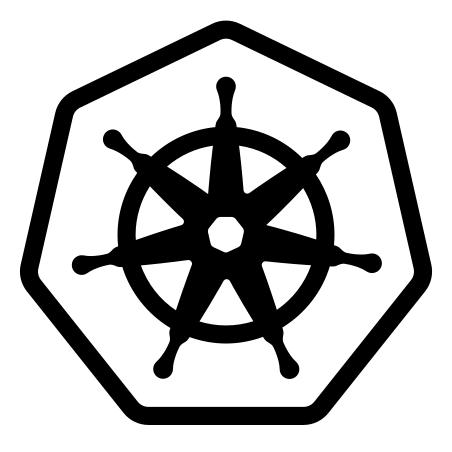
\includegraphics[width=50px]{figures/logos/k8s-bw-2.png}
    \label{fig:abstract:kubernetes}
\end{figure}

\begin{center}
    \large \textbf{\thesisTitle}
\end{center}

{\noindent \textbf{\textsc{Keywords}}}

{\noindent \thesisKeywords}\\


{\noindent \textbf{\textsc{Abstract}}}

\noindent Il \glsname{ml} è una delle branche dell'informatica con le più complesse esigenze computazionali. La difficoltà intrinseca del realizzare modelli di machine learning si amplifica ulteriormente quando sorge la necessità - pressante e inevitabile - di traslare le fasi di sviluppo e di deployment ad un contesto distribuito. Grazie alla sua natura altamente parallelizzabile, i carichi di machine learning sono candidati ideale per i sistemi di orchestrazione di container, che fanno leva sulla scalabilità verticale per assicurare virtualmente un'infinita capacità computazionale.

Nell'ottica di questo lavoro di tesi, due modelli di machine learning dediti all'analisi genomica e realizzati con un paradigma monolitico sono stati sottoposti ad un processo di frammentazione in \glsname{microservizi} containerizzati. Avendo rilevato un sostanziale miglioramento delle performance del modello grazie alla sua nuova architettura, ci si è curati di trasportare la medesima su un cluster Kubernetes in grado di poterne gestire agilmente e con resilienza il ciclo di vita, dall'allenamento alla predizione, orchestrando queste fasi medianti Kubeflow. I risultati ottenuti trovano largo impiego sia su ecosistemi \textit{\glsname{cloudnative}} che \textit{\glsname{bm}}.

Al fine ultimo di tarare l'effettiva possibilità di trasferire in produzione quanto prodotto, è stata condotta un'analisi ad ampio spettro delle possibili vulnerabilità dell'architettura, immaginando molteplici scenari di attacco da parte di un avversario sulla rete. Quest'analisi ha permesso di valutare l'effettiva resilienza del sistema, e di proporre una serie di contromisure atte a mitigare i rischi individuati. Contestualmente, una serie di contributi sperimentali legati alla produzione di immagini Docker e alla loro distribuzione su un cluster Kubernetes sono stati proposti e discussi.

Lo studio condotto sottolinea il ruolo critico di Kubernetes nei sistemi ad alta complessità come quello presentato, ed evidenzia come il paradigma MLOps sia la modalità più organica e competitiva per sfruttare pienamente il potenziale del machine learning mediante l'adozione di architetture scalabili e resilienti con Kubernetes.

Uno spettro di possibili sviluppi futuri è stato osservato contestualmente all'attività progettuale: ad esempio, tecnologie come \glsname{mxnet}, \glsname{ray} o \glsname{mlflow} potrebbero costituire alternative valide a Kubeflow; inoltre, l'integrazione di strumenti di data governance come \glsname{fybrik} consentirebbe l'impiego di dataset contenenti PII, ampliando ulteriormente il campo di applicazione del sistema.

% Publications
%% 
%            ,,                                        
%          `7MM            _.o9                                
%            MM                                             
%  ,6"Yb.    MM  ,p6"bo   ,6"Yb.  M"""MMV  ,6"Yb.  `7Mb,od8 
% 8)   MM    MM 6M'  OO  8)   MM  '  AMV  8)   MM    MM' "' 
%  ,pm9MM    MM 8M        ,pm9MM    AMV    ,pm9MM    MM     
% 8M   MM    MM YM.    , 8M   MM   AMV  , 8M   MM    MM     
% `Moo9^Yo..JMML.YMbmd'  `Moo9^Yo.AMMmmmM `Moo9^Yo..JMML.   
% 
% 
% Free and Open-Source template for academic works
% https://github.com/dpmj/alcazar


% Add here your Publications.
% Depends on Biblatex and Biber for multiple bibliographies.

\newpage
\pagestyle{empty}

\clearpage
\cleardoublepage
\phantomsection

\pagestyle{empty}

% \phantomsection
% \addcontentsline{toc}{chapter}{Publications}


\begin{refsection}

    \nocite{own-article-1, own-article-2, own-article-3}

    \defbibnote{pre-note}{
        \noindent The {\thesisDegree} candidate, {\thesisAuthor}, has co-authored the following publications with Prof. {\thesisTutor} et al. The articles come as a result of the research activities carried out during the {\thesisType}. The candidate is the corresponding author in two of the three publications listed below:
    }
    \defbibnote{post-note}{
        \noindent Note: \cite{own-article-3} is not yet published.
    }

    \printbibliography[heading=bibintoc,  % Title in Table of contents
                       title={Publications},  % Title
                       prenote=pre-note,  % Text before bibliography
                       postnote=post-note]  % Text after bibliography

\end{refsection}


  % Optional: comment this line if you don't need it

% Acknowledgements
%% 
%            ,,                                        
%          `7MM            _.o9                                
%            MM                                             
%  ,6"Yb.    MM  ,p6"bo   ,6"Yb.  M"""MMV  ,6"Yb.  `7Mb,od8 
% 8)   MM    MM 6M'  OO  8)   MM  '  AMV  8)   MM    MM' "' 
%  ,pm9MM    MM 8M        ,pm9MM    AMV    ,pm9MM    MM     
% 8M   MM    MM YM.    , 8M   MM   AMV  , 8M   MM    MM     
% `Moo9^Yo..JMML.YMbmd'  `Moo9^Yo.AMMmmmM `Moo9^Yo..JMML.   
% 
% 
% Free and Open-Source template for academic works
% https://github.com/dpmj/alcazar


% Add here your Acknowledgements. 
% This section is pretty free: free format, in one or various languages, etc.


\newpage
\thispagestyle{empty}

\clearpage
\cleardoublepage
\phantomsection

\pagestyle{plain}

\phantomsection
\addcontentsline{toc}{chapter}{Ringraziamenti}


\vspace*{\fill}

\begin{center}
    \large \textbf{\textsc{Ringraziamenti}}
\end{center}

Questa tesi di laurea magistrale corona il completamento di un percorso accademico quinquennale, disseminato da imprevisti, ostacoli, risultati dolceamari e traguardi che, un tempo, avrei ritenuto irraggiungibili. 

Nonostante l'esito di questo cammino umano e professionale, faccio ancora fatica a definirmi informatico. Durante gli ultimi due anni, ho avuto modo di interfacciarmi con individui di incredibile talento e immensa competenza. Grazie a loro, potrei aver finalmente capito cosa voglio fare nella vita.

Kevin Iuretig, Michele Di Giovanni e Francesco Foglia, con la loro straordinaria intelligenza e dedizione senza pari, hanno segnato il mio cammino professionale in maniera unica e personale. La loro acutissima curiosità e strepitosa intraprendenza hanno acceso la mia passione per il nostro mestiere, guidandomi attraverso sfide e successi. Molto dell'informatico che sono oggi lo devo a loro: per me, è un privilegio potermi considerare loro pari.

Questo percorso non sarebbe stato concretamente e fattualmente realizzabile senza un gruppo coeso e solido, mai sconfitto dal carico di studio né incrinato dal peso degli anni. Mentirei se affermassi che senza Dario Trinchese e Carmine Napolitano, preziosi colleghi e amici, sarei qui oggi a ponderare sul mio percorso post-universitario, poiché probabilmente sarebbe ancora molto distante. Inoltre, è indubbiamente grazie a loro se ho deciso in primo luogo di affrontare il percorso di laurea magistrale; a rendere, sento che non avrei potuto prendere una decisione migliore.

Infine, la mia famiglia, che mi ha sempre sostenuto e incoraggiato, non può che essere considerata la vera protagonista di questo percorso. Senza di loro, non sarei qui oggi a scrivere queste parole. Grazie.

\vspace*{\fill}



% Dedication
% To whom do you dedicate the thesis? Or maybe include a quote, poem, etc. Free space for yourself.
% Delete if you are too manly for these things
%% 
%            ,,                                        
%          `7MM            _.o9                                
%            MM                                             
%  ,6"Yb.    MM  ,p6"bo   ,6"Yb.  M"""MMV  ,6"Yb.  `7Mb,od8 
% 8)   MM    MM 6M'  OO  8)   MM  '  AMV  8)   MM    MM' "' 
%  ,pm9MM    MM 8M        ,pm9MM    AMV    ,pm9MM    MM     
% 8M   MM    MM YM.    , 8M   MM   AMV  , 8M   MM    MM     
% `Moo9^Yo..JMML.YMbmd'  `Moo9^Yo.AMMmmmM `Moo9^Yo..JMML.   
% 
% 
% Free and Open-Source template for academic works
% https://github.com/dpmj/alcazar

\newpage
\thispagestyle{empty}

\clearpage
\cleardoublepage
\phantomsection

\thispagestyle{empty}

\phantomsection
\addcontentsline{toc}{chapter}{Dedication}



\vspace*{\fill}

\begin{flushright}

\textit{\large
\noindent A mia madre}
\end{flushright}



\vspace*{\fill}



% ------------------------------------------------------------------------------
% TABLES OF CONTENTS

\newpage
\thispagestyle{empty}

\clearpage
\cleardoublepage
\phantomsection

\pagestyle{plain}


\begingroup

    % Greatly compress space used by TOC, LOF and LOT
    \renewcommand{\baselinestretch}{1}  % less spacing
    \renewcommand{\contentsname}{Indice dei contenuti}
    \small  % smaller font size
    \setlength{\parskip}{0mm}  % Paragraph skip 0mm

    \pagenumbering{arabic}

    % List of Contents
    {
        %\tableofcontents
        
        %\addcontentsline{toc}{chapter}{Indice dei contenuti}
    }
    
    % List of Figures
    {
        %\listoffigures
        %\addcontentsline{toc}{chapter}{Indice delle figure}
    }
    
    % List of Tables
    {
        %\listoftables
        %\addcontentsline{toc}{chapter}{Indice delle tabelle}
    }
    
    % List of Listings -- uncomment if necessary
    {
        % \listoflistings
        % \addcontentsline{toc}{chapter}{List of listings}

        % \listof{lstlisting}{Code listings} % old code
    }
    
\endgroup

% END OPENING
% ------------------------------------------------------------------------------


